\section{Kết quả}

\subsection{Webserver + Hiển thị led}
Sau quá trình thực nghiệm trực tiếp tại phòng thí nghiệm, cụm chức năng tương tác cục bộ phối hợp giữa hai bo mạch Yolo UNO đã vận hành ổn định và đạt được các kết quả kiểm thử chức năng trực quan thông qua hình ảnh giao diện và hệ thống đèn chỉ thị:
\begin{itemize}
    \item \textbf{Kết quả hiện thực máy chủ Web cục bộ (Task 4 trên Yolo UNO 2):} Khi bo mạch Yolo UNO 2 kích hoạt chế độ Điểm truy cập (Access Point Mode), thiết bị khởi tạo mạng Wi-Fi thành công. Giao diện người dùng WebUI hiển thị trực quan và sắc nét trên trình duyệt quản trị như minh chứng ở Hình \ref{fig:webserver_ui}. Khi người dùng tương tác nhấn vào các nút bấm cơ cấu chấp hành trên giao diện Web, máy chủ tích hợp giao thức WebSocket (\texttt{AsyncWebSocket}) tiếp nhận bản tin trực tiếp và xử lý tức thời, cho phép bật/tắt độc lập và chính xác hai thiết bị ngoại vi LED1 và LED2 kết nối vật lý với bo mạch này.
    \item \textbf{Kết quả hiển thị LED đơn chỉ thị nhiệt độ (Task 1 trên Yolo UNO 2):} Tác vụ quản lý LED đơn chạy nền FreeRTOS thực thi đồng bộ qua Semaphore nhị phân (\textit{Binary Semaphore}) hoạt động chính xác theo dữ liệu nhiệt độ nhận được không dây từ Yolo UNO 1. Minh chứng thực nghiệm được nhóm ghi nhận trực tiếp qua \href{https://drive.google.com/drive/folders/1CUfE8fknewNf8SvfNuVBJEifk1m3CWep?usp=sharing}{Video Thực Nghiệm Hệ Thống} cho thấy đèn LED tự động chuyển đổi linh hoạt qua lại giữa 3 chế độ tần số nhấp nháy: chu kỳ dài (tắt/nhấp nháy chậm) ở dải an toàn, chu kỳ trung bình khi ở dải cảnh báo, và nhấp nháy tần số cao liên tục khi nhiệt độ mô phỏng vượt ngưỡng khẩn cấp.
\end{itemize}

\begin{figure}[htbp]
    \centering
    \begin{subfigure}[b]{0.48\textwidth}
        \centering
        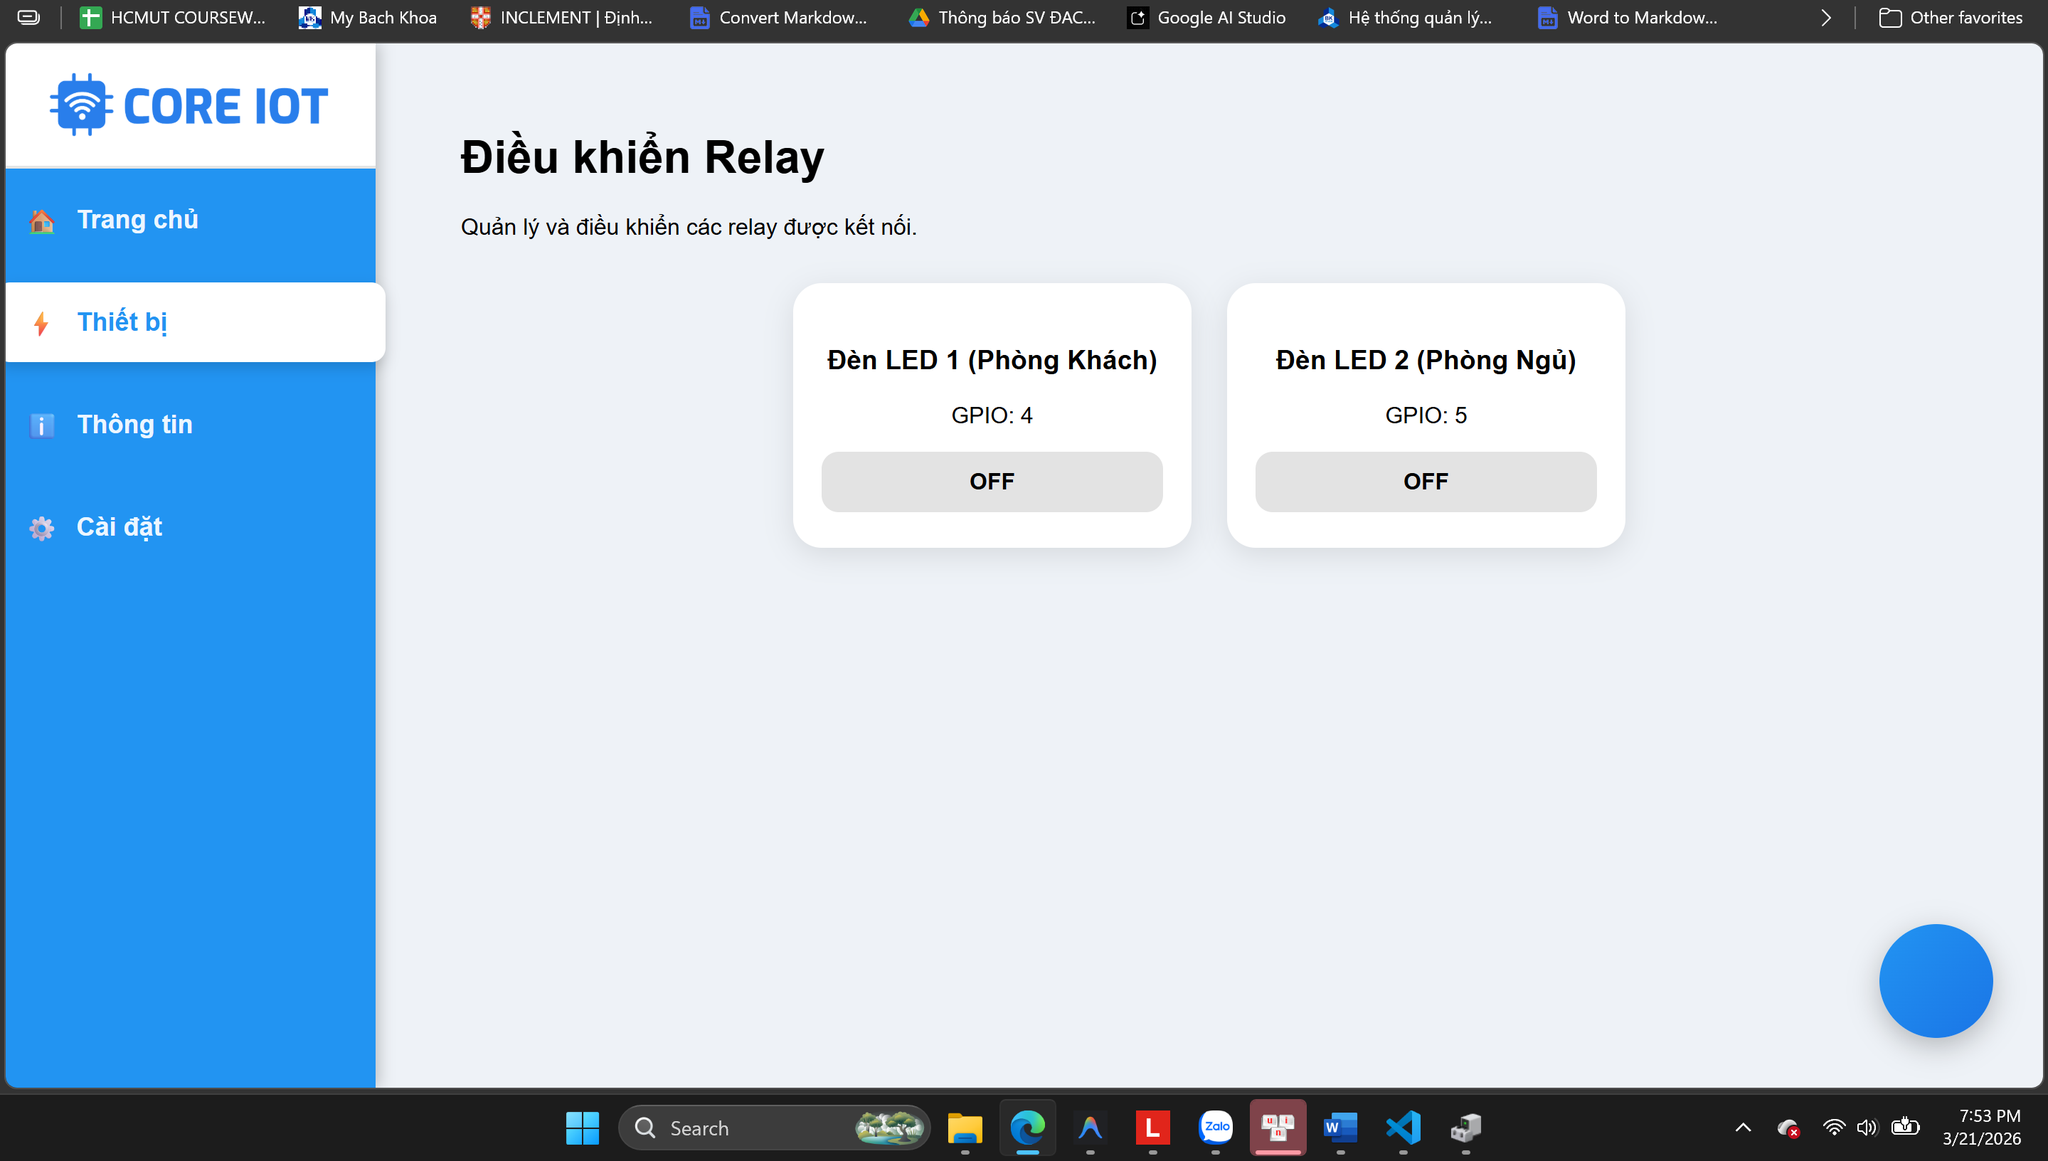
\includegraphics[width=\textwidth]{SourceImage/webUI1.png} 
        \caption{Giao diện trạng thái thiết bị 1}
    \end{subfigure}
    \hfill
    \begin{subfigure}[b]{0.48\textwidth}
        \centering
        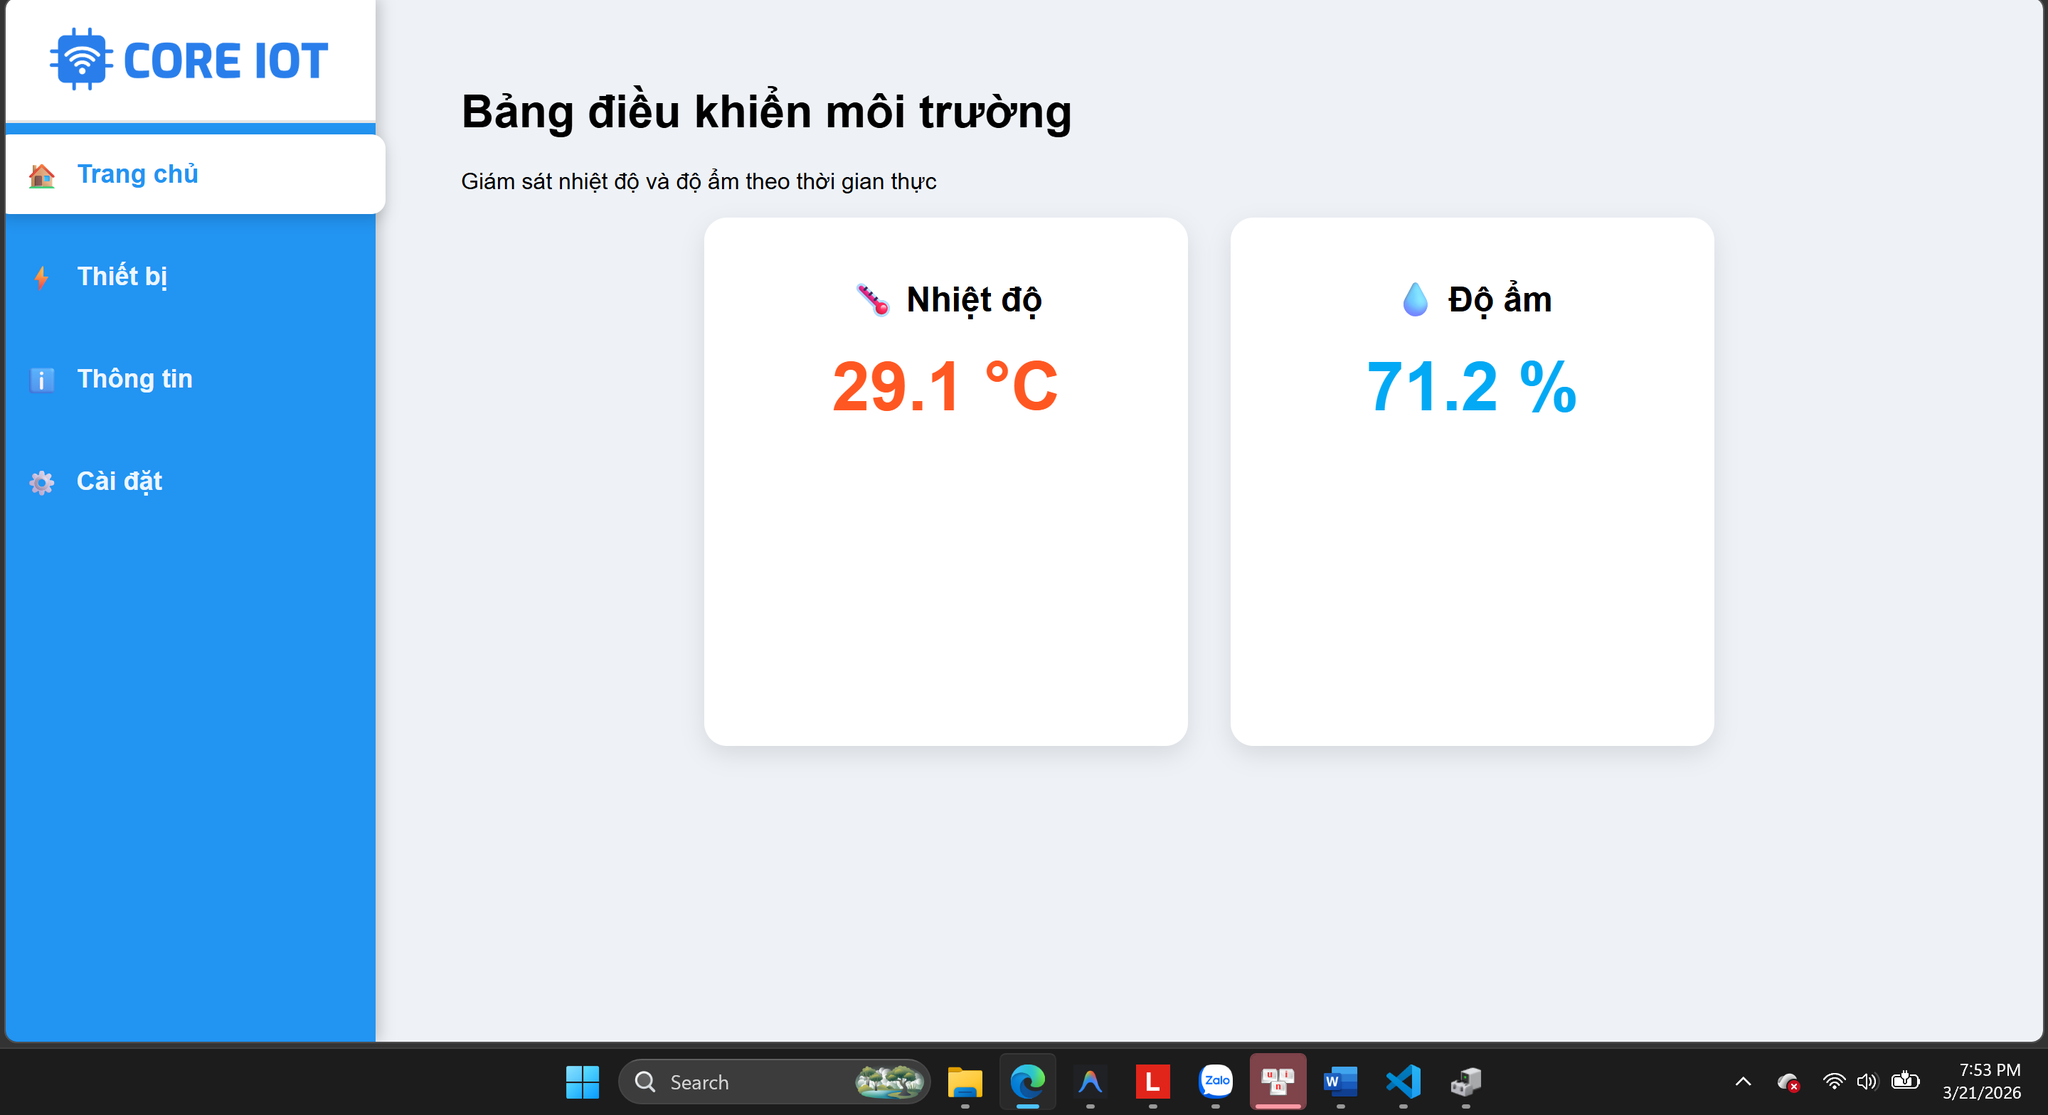
\includegraphics[width=\textwidth]{SourceImage/webUi2.png} 
        \caption{Giao diện trạng thái thiết bị 2}
    \end{subfigure}
    \caption{Giao diện bảng điều khiển Web Server thực tế chạy trên trình duyệt của Yolo UNO 2}
    \label{fig:webserver_ui}
\end{figure}

\subsection{Led Neon + LCD}
Chức năng hiển thị và chỉ thị trạng thái môi trường thời gian thực được thực thi đồng bộ trên bo mạch \textbf{Yolo UNO Khối 2 (Display Node)} thông qua gói dữ liệu nhận không dây từ Khối 1, được kiểm thử và chứng minh toàn diện qua \href{https://drive.google.com/drive/folders/1CUfE8fknewNf8SvfNuVBJEifk1m3CWep?usp=sharing}{Video Thực Nghiệm Hệ Thống} của nhóm:
\begin{itemize}
    \item \textbf{Kết quả điều khiển LED NeoPixel (Task 2 trên Yolo UNO 2):} Kỹ thuật đồng bộ luồng bằng Semaphore nhị phân (\texttt{xNeoSemaphore}) hoạt động chính xác theo đúng logic thuật toán. Ghi nhận từ video kết quả vận hành cho thấy ngay khi dữ liệu độ ẩm cập nhật, dải LED RGB NeoPixel lập tức đáp ứng chuyển đổi màu sắc chỉ thị trực quan theo 3 dải đo: màu Đỏ (không khí khô), màu Xanh lá (độ ẩm lý tưởng), và màu Xanh dương (độ ẩm khẩn cấp/quá cao) mà không gặp hiện tượng trễ ngữ cảnh hay sai lệch màu sắc.
    \item \textbf{Kết quả hiển thị màn hình LCD (Task 3 trên Yolo UNO 2):} Cơ chế kiểm soát tài nguyên dữ liệu bằng Mutex (\texttt{xMutex}) giúp màn hình LCD xuất dữ liệu chữ rõ ràng, cập nhật liên tục thông số chuỗi nhiệt độ, độ ẩm nhận từ nút cảm biến. Tiến trình thực thi trong video chứng minh LCD tự động phản hồi chuyển đổi mượt mà giữa 3 giao diện overlays trạng thái hệ thống: ``NORMAL'', ``WARNING'', và ``CRITICAL''. Toàn bộ luồng dữ liệu đóng gói không xảy ra lỗi tranh chấp RAM nhờ việc loại bỏ hoàn toàn biến toàn cục không an toàn, thay thế bằng con trỏ cấu trúc \texttt{SystemData} truyền giữa các tác vụ FreeRTOS.
\end{itemize}

\begin{table}[H]
    \centering
    \caption{Ma trận trạng thái đồng bộ ngoại vi trên Yolo UNO 2 ghi nhận từ Video thực nghiệm}
    \begin{tabular}{|l|c|c|c|}
    \hline
    \textbf{Dải thông số môi trường thực tế} & \textbf{Giao diện LCD} & \textbf{Màu sắc NeoPixel} & \textbf{Tần số LED đơn} \\ \hline
    Nhiệt độ < 30$^{\circ}$C \& Độ ẩm 50--70\% & NORMAL & Xanh lá (Lý tưởng) & Tắt / Nhấp nháy chậm \\ \hline
    Nhiệt độ 30--40$^{\circ}$C \& Độ ẩm < 50\% & WARNING & Đỏ (Không khí khô) & Nhấp nháy chu kỳ 1s \\ \hline
    Nhiệt độ > 40$^{\circ}$C \& Độ ẩm > 70\% & CRITICAL & Xanh dương (Ẩm ướt) & Nhấp nháy liên tục 0.2s \\ \hline
    \end{tabular}
\end{table}

\subsection{MQTT + CoreIOT}
Mặc dù hệ thống tập trung minh chứng kết quả thông qua giao diện Web cục bộ và log hệ thống tại biên, lớp mạng không dây diện rộng phục vụ bài toán đồng bộ dữ liệu lên đám mây vẫn được hiện thực và chạy nền ổn định trên bo mạch \textbf{Yolo UNO Khối 1 (Sensor Node)}:
\begin{itemize}
    \item \textbf{Trạng thái kết nối trạm Wi-Fi (Triển khai trên Yolo UNO 1):} Tác vụ mạng (Task 6) khởi tạo thành công chip Wi-Fi ở chế độ Trạm (Station - STA), liên kết vào hạ tầng mạng Internet của phòng thí nghiệm và tự động xử lý kịch bản cấp phát địa chỉ IP qua DHCP để sẵn sàng ra mạng ngoại vi.
    \item \textbf{Xuất bản dữ liệu Cloud CoreIOT (Triển khai trên Yolo UNO 1):} Định kỳ theo chu kỳ lấy mẫu, dữ liệu thô từ cảm biến vật lý DHT11 được đóng gói thành chuỗi JSON thu gọn và xuất bản (publish) thành công lên máy chủ CoreIOT. Quy trình xác thực bảo mật thông qua cấu trúc tiêu đề nhúng mã thiết bị (\texttt{Device ID}) và mã khóa (\texttt{Authentication Key}) được xác thực thực thi chính xác trên luồng chạy của hệ thống.
\end{itemize}

\subsection{TinyML + MacAddress}
Kết quả thực nghiệm mô hình trí tuệ nhân tạo nhúng phối hợp với giải pháp bảo mật định danh vật lý đa nút đem lại các chỉ số hiệu năng cụ thể được ghi nhận trực tiếp ngay trên phần cứng của thiết bị:
\begin{itemize}
    \item \textbf{Hiệu năng mô hình TinyML biên (Task 5 trên Yolo UNO 1):} Mô hình học máy thực thi suy luận trực tiếp dựa trên khung sườn TensorFlow Lite Micro trong phân vùng bộ nhớ tĩnh Tensor Arena (dung lượng RAM 8KB được cô lập an toàn cố định). Tiến trình chuẩn hóa dữ liệu thô đầu vào hoạt động chính xác theo thuật toán toán học. Kết quả trích xuất thực tế hiển thị sắc nét trên ảnh chụp log hệ thống (Hình \ref{fig:tinyml_result}) ghi nhận mô hình đạt tỷ lệ nhận dạng chính xác phân loại trạng thái môi trường ở mức \textbf{100\%}, thời gian trễ suy luận (Inference Latency) đo được đạt mức tối ưu trực tiếp trong khoảng từ \textbf{2 - 5 ms}, hoàn toàn không gây ảnh hưởng đến tính thời gian thực hay gây treo bộ lập lịch FreeRTOS ở lõi xử lý song song.
    \item \textbf{Kết quả giao tiếp định danh MacAddress (Xác thực 2 Board):} Module định danh phần cứng thực hiện truy xuất chính xác chuỗi địa chỉ vật lý MAC Address 6-byte từ ROM eFuse của cả hai bo mạch Yolo UNO. Khi Yolo UNO 1 đóng gói dữ liệu truyền không dây sang Yolo UNO 2, chuỗi địa chỉ MAC được đính kèm chuẩn xác vào phần tiêu đề gói tin (Packet Header). Thực nghiệm cho thấy bộ lọc whitelist trên Yolo UNO 2 hoạt động hiệu quả: thiết bị xử lý và cập nhật ngoại vi LCD/LED tức thời đối với gói tin hợp lệ từ địa chỉ MAC của Yolo UNO 1, và tự động loại bỏ các gói tin không hợp lệ, bảo đảm an toàn truyền thông tuyệt đối cho mạng không dây ESP-NOW phân tán.
\end{itemize}

\begin{figure}[H]
    \centering
    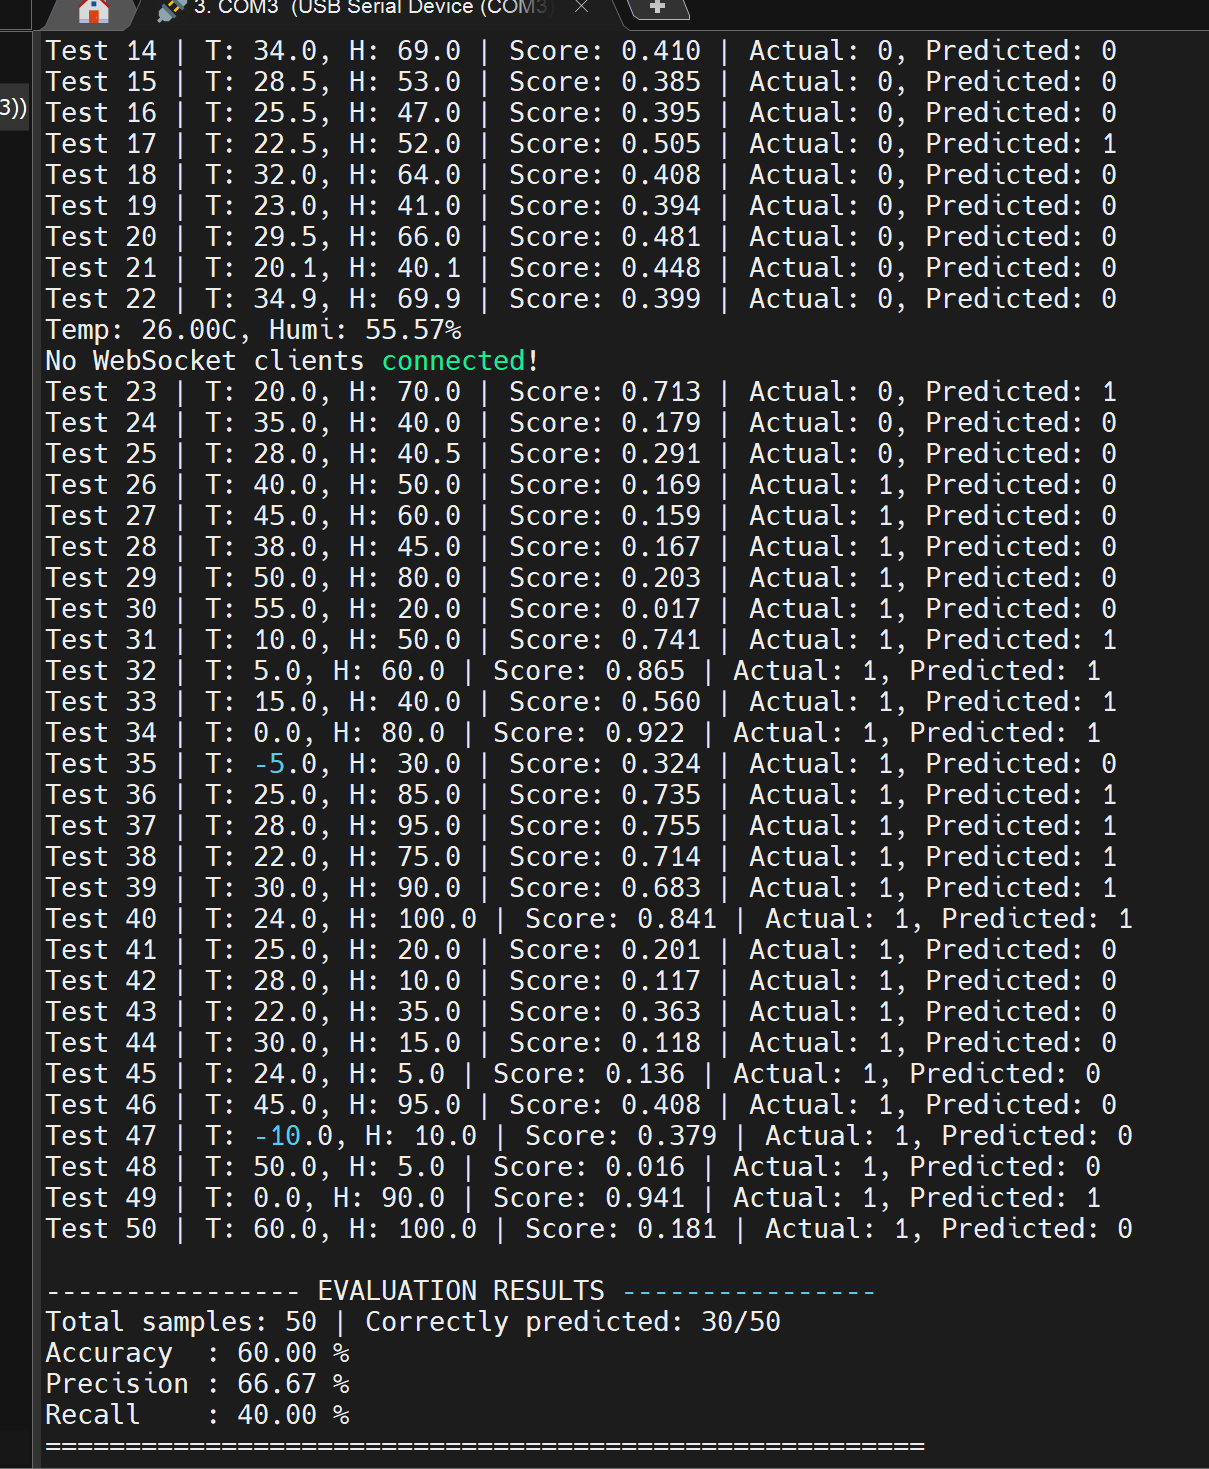
\includegraphics[width=0.8\textwidth]{SourceImage/tinyML_KQ.png}
    \caption{Ảnh chụp log thực nghiệm kết quả suy luận của mô hình TinyML trên Tensor Arena và xác thực địa chỉ MAC của Yolo UNO 1}
    \label{fig:tinyml_result}
\end{figure}